\section{RationalGRL evaluation experiment}
\label{sect:validation}

In addition to the empirical case study (Section~\ref{sect:gmas}), which forms the basis of the RationalGRL framework, we also performed a user evaluation with 16 users. The objective of this evaluation was to determine whether the users found the additions of RationalGRL (arguments, argumentation semantics, critical questions) useful compared to standard GRL, and whether they found it easier to keep track of and express opinions and beliefs using RationalGRL compared to standard GRL. Regarding the comparison of RationalGRL to GRL, the following two broad hypotheses follow from our main points in this paper:

\begin{itemize}
\item[H1] The additions of RationalGRL -- arguments, critical questions and determination of the status of arguments -- are a useful addition to standard goal modelling in GRL.
\item[H2] The additions of RationalGRL make it easier to express, determine the effect of and communicate to other stakeholders one's opinions and beliefs about a goal model.
\end{itemize}

In addition, we wanted to know whether the RationalGRL tool was difficult or easy to use. Note that we did not aim to conduct a usability study for the RationalGRL tool. Rather, we were interested to know if the tool was clearly very easy or difficult to use, as this could influence the participants ideas about the RationalGRL framework and language -- a very nice and easy to use tool tends to make people more positive towards a particular modelling language, whereas irritations about a bad tool will lead to a more negative disposition. This leads to the following general hypothesis:

\begin{itemize}
\item[H3] The usability of the RationalGRL tool is neither (very) easy or (very) difficult. 
\end{itemize}

In the rest of this section, we will describe our experiment in more detail and further specify these hypotheses.

\subsection{Experiment design}

The idea was to have our participants perform a small modelling task, and then ask them what they thought of RationalGRL and the tool. Thus, our experiment consisted of three parts:

\begin{enumerate}
\item Explanation: We explain to the participants the basics of the RationalGRL development process and the RationalGRL tool.
\item Modeling: We ask the participants to model a summarized discussion in the RationalGRL tool.
\item Survey: We present the participants with a survey containing questions about the comparison between RationalGRL and GRL, and questions about the usability of the RationalGRL tool.
\end{enumerate}

The instructions for these three parts are contained in a single document that we sent out to the participants.\footnote{See \url{www.rationalgrl.com}, page ``Empirical Study''} The explanation (part 1) starts with a general explanation of GRL and standard goal modelling similar to the explanation provided in section \ref{{sect:background:grl}, then briefly discusses the additions of RationalGRL (argument, attack, critical questions) and finally the tool is briefly described (similar to Section \ref{sect:tool}). 

For part 2, we provided a small part of a transcript and some context information (see Appendix~\ref{sect:survey}) and asked the participants to model this in the tool and take a screenshot of their final model. The idea is that the participants act as if they are ``present'' at a discussion about the early-stage requirements and are asked to model the goal model corresponding to these requirements. 

For part 3, we provided the participants with a survey\footnote{https://goo.gl/forms/fDSMUnAV20wy7kbY2}. The survey starts with general questions about the participant (experience etc.). It then asks the following questions about the RationalGRL tool, asking the participants to rate various aspects of the tool on a Likert scale of 1 (very difficult) to 5 (very easy):
\begin{itemize}
\item[Q1] Was it easy or difficult to get started with the RationalGRL tool?
\item[Q2] Was the details pane (containing details of an element, critical questions, etc) easy or difficult to use?
\item[Q3] Was it easy or difficult to understand the way in which the status of arguments and other elements is determined?
\item[Q4] Did you find it easy or difficult to model the example discussion using RationalGRL?
\end{itemize}
We also ask open questions about the strengths and weaknesses of the tool, possible improvements and whether the participant thinks the tool could in the future be used in practice.

The second part of the survey concerns the comparison between GRL and RationalGRL and starts with Figure~\ref{fig:example-small}, which models the discussion for part 2 (Appendix~\ref{sect:survey}) in standard GRL, so that the participants can compare their own RationalGRL models and experiences with the standard GRL model. The following questions ask the participants to rate RationalGRL on a Likert scale from 1 (very useless) to 5 (very useful):
\begin{itemize}
\item[Q5] Do you think the arguments and counterarguments of RationalGRL are a useful extension to standard goal modeling?
\item[Q6] Do you think the critical questions and answers in the details pane are a useful extension to standard goal modeling?
\item[Q7] Do you think the automatic determination of the status of arguments and elements is a useful extension to standard goal modeling?
\end{itemize}
The following questions ask the participants to rate RationalGRL vs. standard goal modelling on a Likert scale from 1 (much more difficult) to 5 (much easier):
\item[Q8] Do you think using RationalGRL instead of a standard goal modeling language makes it easier or more difficult to for someone to express beliefs and opinions in a goal model?
\item[Q9] Do you think using RationalGRL instead of a standard goal modeling language makes it easier or more difficult to for someone to determine the effect of beliefs and opinions on the resulting goal model?
\item [Q10] Do you think using RationalGRL instead of a standard goal modeling language makes it easier or more difficult to for someone who is not the original author to understand the goal model? 
\end{itemize}
We conclude with two open questions regarding the strengths and weaknesses of RationalGRL compared to GRL.

In order to test our main hypotheses H1, H2 and H3, we have to formulate the appropriate null hypotheses and alternative hypotheses. For H1 and H2, we hypothesize that the participants will, on average, rate the additions of RationalGRL as useful (rating 4) or very useful (rating 5) for Q5, Q6 and Q7, and as making it easier (rating 4) or significantly easier (rating 5) for questions Q8, Q9 and Q10. In other words, we say that our null hypothesis and alternative hypothesis for H1 and H2 are as follows:
\begin{itemize}
[] H1$_{0}$ and H2$_{0}$: average rating for questions Q5-Q10 is 3 or lower.
[] H1$_{a}$ and H2$_{a}$: average rating for questions Q5-Q10 is higher than 3.
\end{itemize}
Note that for each question (Q5-Q10) we can test the null and alternative hypothesis separately, giving insight into exactly which additions of RationalGRL were deemed useful. 

For hypothesis H3, we do not claim that the usability of the tool is especially easy or difficult: we expect the average rating for questions Q1-Q4 to not be significantly higher or lower than 3 (neither easy or difficult). Thus, our null hypothesis and alternative hypothesis for H3 are as follows:  
\begin{itemize}
[] H3$_{0}$: average rating for questions Q1-Q4 is 3.
[] H3$_{a}$: average rating for questions Q1-Q4 is not 3.
\end{itemize}
Again, we can test these hypothesis separately for each of the questions.

\paragraph{Participants}
We asked 16 participants in our network to participate in our experiment. Most of the participants were therefore either employed at the first author's company or staff and (ex-)students from the second author's university. Hence, two thirds of the participants had either a PhD or Master degree, 20\% a Bachelor degree, and one respondent responded with ``Other''. All but one participant had a year or more experience with software development. The average experience was 6.2 years (standard deviation 6.7), with 10 participants having less than 5 years of experience and 6 participants having 8 or more years of experience, with one participant having 25 years of experience. The participants also judged themselves to be quite competent in  early-phase requirements engineering: on average they gave themselves a rating of 3.2 out of 5 (standard deviation 1.3) with half of the participants claiming they were at least ``competent'' (rating 4) or ``very competent'' (rating 5). However, experience with goal modeling languages was markedly less: the average rating was 1.9 (standard deviation 1.3), with 9 participants claiming never to have used a goal modeling language (rating 1), and only two participants displaying regular use (monthly, rating 4, or weekly, rating 5). The participants that had experience with goal modelling languages had mostly used i* (5 users), with 2 users being familiar with GRL and 2 users having used another goal modelling language.

\subsection{Results}\label{sec:survey:results}

\begin{table*}[t]
\centering
\begin{tabularx}{0.95\textwidth}{l|l|l|l|l|l|l|l}
& very difficult & difficult & neither difficult nor easy & easy & very easy & avg. score (1-5) & std. dev.\\
\hline
Q1 & 2 (12.5\%) & 1 (6.3\%) & 6 (37.5\%) & 6 (37.5\% & 1 (6.3\%) & 3.2 & 1.1\\
Q2 & 2 (12.5\%) & 2 (12.5\%) & 4 (25\%) & 8 (50\%) & 0 (0\%) & 3.1 & 1.1\\
Q3 & 0 (0\%) & 3 (20\%) & 4 (26.7\%) & 5 (33.3\%) & 3 (20\%) & 3.5 & 1.1\\
Q4 & 2 (12.5\%) & 5 (31.3\%) & 6 (37.5\%) & 3 (18.8\%) & 0 (0\%) & 2.6 & 1.0
\end{tabularx}
\caption{User scores for the usability of the RationalGRL tool}
\label{table:survey:table1}
\end{table*}

\begin{table*}[t]
\centering
\begin{tabularx}{0.95\textwidth}{l|l|l|l|l|l|l|l}
& very useless & useless & neither useful nor useless & useful & very useful & avg. score (1-5) & std. dev.\\
\hline
Q5 & 0 (0\%) & 0 (0.0\%) & 3 (21.4\%) & 8 (57.1\% & 3 (21.4\%) & 4.0 & 0.7\\
Q6 & 0 (0.0\%) & 3 (21.4\%) & 3 (21.4\%) & 6 (42.9\%) & 2 (14.3\%) & 3.5 & 1.0\\
Q7 & 0 (0\%) & 0 (0\%) & 2 (14.3\%) & 7 (50.0\%) & 5 (35.7\%) & 4.2 & 0.7
\end{tabularx}
\caption{Participant ratings of the usefulness of the additions of RationalGRL}
\label{table:survey:table2}
\end{table*}

\begin{table*}[t]
\centering
\begin{tabularx}{0.95\textwidth}{l|l|l|l|l|l|l|l}
& much more difficult & more difficult & neither more difficult nor easier & easier & much easier & avg. score (1-5) & std. dev.\\
\hline
Q8 & 0 (0\%) & 0 (0.0\%) & 3 (21.4\%) & 8 (57.1\% & 3 (21.4\%) & 4.0 & 0.7\\
Q9 & 0 (0.0\%) & 3 (21.4\%) & 3 (21.4\%) & 6 (42.9\%) & 2 (14.3\%) & 3.5 & 1.0\\
Q10 & 0 (0\%) & 0 (0\%) & 2 (14.3\%) & 7 (50.0\%) & 5 (35.7\%) & 4.2 & 0.7
\end{tabularx}
\caption{Participant ratings of whether the additions of RationalGRL make reasoning about a goal model easier **MARC PLEASE FILL IN THE CORRECT NUMBERS FROM THE SURVEY HERE, TNX}
\label{table:survey:table3}
\end{table*}

First, the participants had to perform the modeling task. They produced RationalGRL models containing on average 3 arguments (in addition  to goals, tasks, etc.) from the short transcript. Some of the examples of RationalGRL models the users created can be found in Appendix~\ref{sect:survey-screenshots}.

After the modelling task, the survey questions were asked. Table~\ref{table:survey:table1} shows the respondents' answers, the average score, and the standard deviation for questions Q1-Q4. 
We also asked the users three open questions related to usability. When asked about the strengths and weaknesses of the RationalGRL tool, users where generally positive about RationalGRL's clear UI, the fact that the tools gives a nice overview of the goals and opinions in a case and that it was straightforward to use and understand. With respect to weaknesses and improvements to the RationalGRL tool, the users mentioned additional UI functionalities such as the possibility to save models, having an ``undo'' function, and flipping the arrow after adding them. Users also suggested various language-related improvements. Some users mentioned they missed the possibility to attack links, while others mentioned that not all GRL elements are supported (for instance, it is currently not possible to add actors).

When asked in an open question whether the users believe a more mature version of the RationalGRL tool could be used to capture early-phase requirements in an actual software development project, most users responded positively. Users' responses include ``Yes, having the possibility to add arguments seems quite useful'', ``I think it can, but maybe try to find a way to combine it with more regular/mainstream requirements gathering such as user stories and customer journeys'', ``yes, because it creates a clear scope for the project, what the goals are'', and ``Generally I think its useful to explicitly document arguments of a discussion''. The concern that the modeling process may involve too much cognitive overhead was mentioned a few times though: ``I think the overhead of inputting a (detailed) discussion in a structured manner into any system makes adoption difficult'', ``the manual input is too complex and takes too much time. An automated process of parsing the conversation log would be much more helpful'', and ``I still believe in the value of arguments, but there should be less confusing ways to capture them''.

Tables~\ref{table:survey:table2} and \ref{table:survey:table3} show the respondents' answers, the average score, and the standard deviation for questions Q5-Q7. We concluded with two open questions about the comparison between RationalGRL and other goal modeling languages. When asked about the advantages of RationalGRL over standard goal modeling languages, many users agreed that making arguments explicit may force end users to have a more structured discussion: ``	Clear communication about argumentation and forcing people to think in those clear terms.'', ``...you can add arguments and that you can answer questions that help you to develop arguments'', ``It's useful that discussion and explanation are close to the diagrams'', ``a way to see how decisions are being shaped.''. Furthermore, one user stated that RationalGRL successfully ``tries to capture the rationale behind the modeling process' and ``has a simple way to compute the status of the arguments''. When asked about the weaknesses, users mentioned the complexity as the most important weakness: ``The apparent increase in complexity might lead to negative perceptions'', ``adding yet another layer of complexity scares me''. One user mentioned that this may be a problem with goal modeling in general: ``Goal models are already complex (...) I have worked for years on the effect of context on goal models, and my conclusion is that this was very interesting academic work but with close-to-zero practical implications, unfortunately.''.

\subsection{Analysis and discussion}

\paragraph{Hypothesis H1}
The first analysis concerns hypothesis H1, whether the additions of RationalGRL -- arguments, critical questions and determination of the status of arguments -- are a useful addition to standard goal modelling in GRL. Table~\ref{fig:statsanalysis1} summarizes the average scores, standard deviations, p-values for a right-tailed t-test, effect size and statistical power for the relevant questions Q5-Q7. As can be seen, all the averages are significantly higher than the median of 3 with a significance level ($\alpha$) of 0.05, which means that we can accept H1$_{a}$ and reject H1$_{0}$ for all the separate questions Q5-Q7. In other words, the fact that the participants rate the additions of RationalGRL as, on average, (very) useful is very unlikely to be due to chance. 

For questions Q5 and Q7, the effect sizes are very large\footnote{Where am low p-value indicates whether the fact that average rating of a question is statistically significantly higher than the median 3, the effect size indicates the magnitude of the difference between the measured average and the median. Generally, an effect size below 0.2 is seen as low, and effect size of 0.5 is seen as medium, an effect size of 0.8 is seen as large and an effect size of 1.2 is seen as very large.}. This means that the addition of arguments and the use of arguments to determine the acceptability of elements of the goal model are deemed to be useful to very useful by the participants. This can also be seen in Table~\ref{table:survey:table2}: no participant found the addition of arguments and argument status useless or very useless, and 78.6\% (Q5) respectively 85.7\% (Q7) found the additions useful or very useful. Furthermore, these findings fit with the answers to the open questions (see Section \ref{sec:survey:results}). Finally, the statistical power for these questions is very high (>0.99), which means that the chances of wrongly rejecting H1$_{0}$ are close to 0. 

Interestingly, while for Q6 the average is significantly higher than the median 3, the effect size is only medium and the power is not very high, with the chances of wrongly rejecting H1$_{0}$ being almost 50\%. Hence, we can say that the addition of critical questions is perhaps not as useful as we had hypothesized. This again fits the descriptive statistics in Table\ref{table:survey:table2}: 21.4\% of respondents found the critical questions ``useless''. Furthermore, in the open questions a number of participants indicated that the exact difference between some of the critical questions was unclear, and that some of the critical questions seemed unnecessary, at least for the small modeling exercise given in the experiment.

\paragraph{Hypothesis H2}
The second hypothesis states that additions of RationalGRL make it easier to express one's opinions and beliefs about a goal model, determine the effect of one's opinions and beliefs about a goal model and communicate one's opinions and beliefs about a goal model to other stakeholders. Table~\ref{fig:statsanalysis1} again provides a summary of the statistical analysis of the relevant questions Q8-Q10. As can be seen, all the averages are significantly higher than the median of 3 with a significance level ($\alpha$) of 0.05, which means that we can accept H1$_{a}$ and reject H1$_{0}$ for all the separate questions Q8-Q10. In other words, the fact that the participants rate the additions of RationalGRL as making it, on average, easier to reason with their beliefs and opinions about a goal model is very unlikely to be due to chance. 

With respect to Q8, there is again a very large effect size and high statistical power: participants say that arguments make it much easier to express their opinions. None of the participants found expressing their beliefs (much) more difficult, and 69.3\% found it easier or much easier. This corresponds to the answers to Q5, where participants said the arguments were a useful addition. Like for Q5, for Q8 the chances of wrongly rejecting H1$_{0}$ are close to 0. 

For Q9, the effect size is somewhat smaller, though still large: RationalGRL makes it easier to determine the effect of one's beliefs on the goal model. Power shows that there is a small (around 7.5\% chance) or wrongly rejecting the null hypothesis. However, combining this with the results for question Q7, which asked about the usefulness of determining the status, we can say that the participants overall found this a useful feature which makes working with conflicting beliefs easier. One participant remarked that ``The reasoning [in the example] seems simplistic [...] the added value of [the formal argumentation] would be justified if the reasoning is more complex''. So the simplistic case in the modeling exercise possibly detracts from the results for Q9 and Q7.

The analysis of the results for Q10 show a medium to large effect size: overall, participants were less sure that arguments would help in communicating the goal model to others. Statistical power is also not that high at 77\%. This may be due to the fact that in the experiment, communication of opinions to others was not really tested, leaving the participants to guess what this effect would be.  

\paragraph{Hypothesis H3}
\begin{figure}[t]
\centering
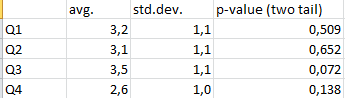
\includegraphics[width=\textwidth]{img/Table_analysisQ1-Q4.png}
\caption{Statistical analysis of the results of Q1-Q4 **MARC CAN YOU CONVERT THIS INTO A PROPER LATEX TABLE? THANKS!}
\label{fig:statsanalysis2}
\end{figure}

On average, the participants did not find the tool easy or difficult to use, with most average scores being between 2.5 and 3.5. There were a number of users that had some trouble getting started (in 3 out of the 4 questions, 12.\%5 rated ``very difficult''). We think this is not unexpected, as the cognitive burden for our framework is higher than for other goal modeling languages such as GRL and i*, simply because there are more elements in the language. 




\subsection{Analysis}\label{sec:eval-an}
Although our empirical evaluation is relatively small-scale, and we cannot draw hard conclusions from it, we do believe that we can extract some interesting observations. We list the three most important ones:
\begin{enumerate}
\item \emph{High cognitive overhead.} A concern that was raised often in our empirical evaluation is that, in its current form, RationalGRL has a relatively high cognitive overhead. Goal modeling is by itself already a cognitively high-effort activity, and the fact that we add more elements to the language does not improve this. This may mean that in future work we should focus more on the RationalGRL development process\footnote{Note that in order to keep the study simple for the users, we did not explicitly ask the respondents to follow the development process from Section~\ref{sect:methodology}}. Users like to be guided during modeling phase, and making arguments explicit in the modeling process was indicated as useful, but argumentation should be integrated into the \emph{process} of goal modeling more than in the goal models themselves. Critical questions seem to be a natural fit for this, as they play a key role in the RationalGRL development process, but in its current form they are only mentioned in the details pane of the tool.
\item \emph{Useful argumentation semantics.} Participants were enthusiastic about adding arguments to a goal modeling language with a clear formal underpinning, and they believed the argumentation semantics we use in the tool is very intuitive. This is a positive signal for our formal approach.
\item \emph{Lightweight tool.} Respondents were positive about the fact that it was very easy to get started with the tool. Thus, it seems that having a simple web-interface for goal modeling languages is something that could be done more in the future. Most comments on the tool were the type of comments that are expected from a prototype implementation.
\end{enumerate}